\begin{figure*}[t]
    \centering
    \begin{subfigure}[t]{0.49\linewidth} % <--- [t] per top alignment
        \centering
        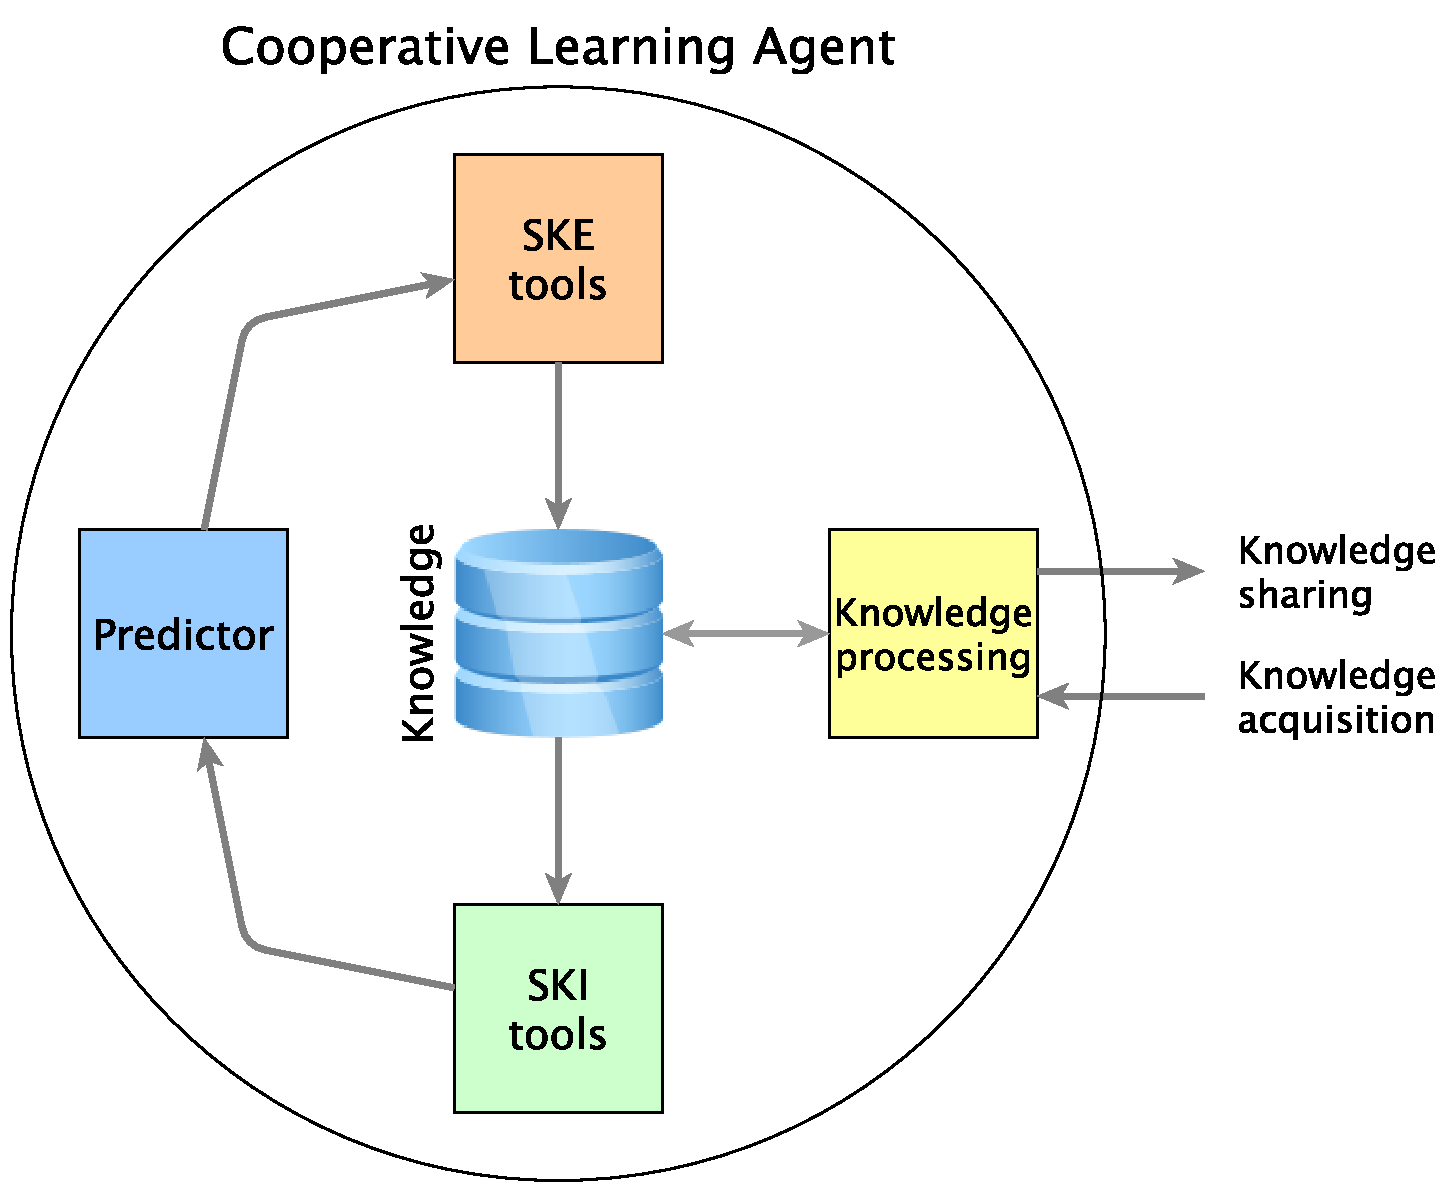
\includegraphics[width=\linewidth]{figures/cl-agent}
        \caption{
            Agent's architecture for \gls{CoL}.
            %
            The agent is equipped with a set of \gls{SKE} and \gls{SKI} methods to manipulate knowledge, plus some functions to pre/post-process knowledge.
        }
        \label{fig:cl-agent-architecture}
    \end{subfigure}%
    \hfill
    \begin{subfigure}[t]{0.49\linewidth} % <--- [t] per top alignment
        \centering
        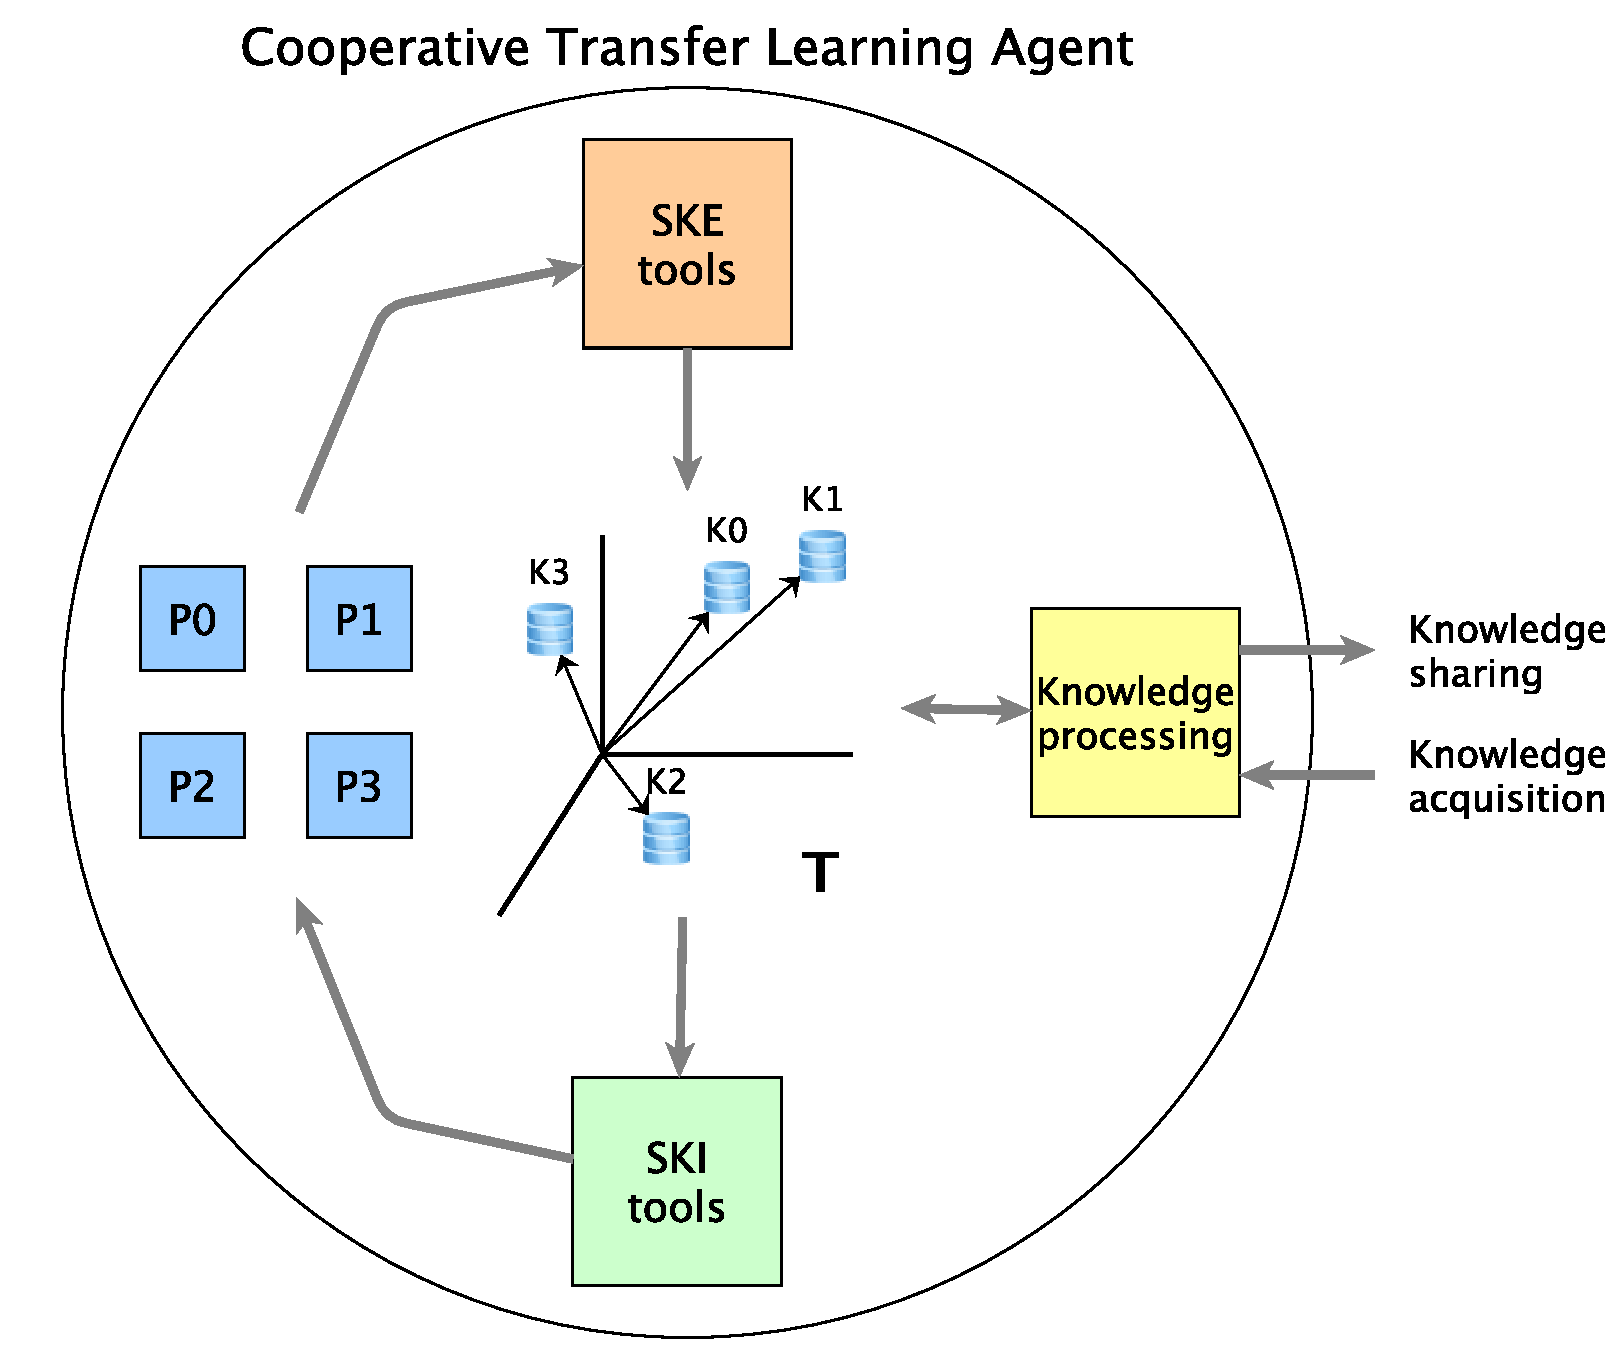
\includegraphics[width=\linewidth]{figures/ctl-agent}
        \caption{
            Agent's architecture for \gls{CoTL}.
            %
            The agent is equipped with a set of \gls{SKE} and \gls{SKI} methods to manipulate knowledge, functions to pre/post-process knowledge, plus a task space and relatedness functions to evaluate if two different tasks are related.
            %
            Each task in the task space $T$ is paired with its specific knowledge. For each task the agent has at least one predictor.
            %
            In the example are represented the knowledge of four tasks but they can come in arbitrary number.}
        \label{fig:ctl-agent-architecture}
    \end{subfigure}
    \caption{Architectures for \gls{CoL} and \gls{CoTL} agents.}
    \label{fig:architectures}
\end{figure*}
